%!TEX root = ../../../../exa-ma-d7.1.tex

\section{Mini App: Test I/O at large scale}


This mini application tests the input and output of data for \Feelpp.
\Cref{tab:app-feelpp-io} describes the specifications of the application.

\begin{table}[ht]
    \centering
    \begin{tblr}{
        colspec = {l X[10cm]},
        row{odd} = {numpexlightergray},
        hlines = {0.1pt, numpexgray},
        vlines = {numpexgray},
        row{1} = {numpexgray, fg=white, font=\bfseries},
    }
        Field & Details \\
        id & \texttt{app-feelpp-io} \\
        name & Test I/O at large scale \\
        Partners &  Unistra \\
        PC & PC1 - ExaMA, PC2 - WP2 \\
        Responsible (Permanent) &  V. Chabannes, C. Prud'homme \\
        WP7 Engineer & Thomas Saigre (UNISTRA) \\
        work\_package & WP1 \\
        application\_type & mini-app \\
        % purpose & \\
        % Method-Algorithm WP1 & \\
        % Method-Algorithm WP2 & \\
        % Method-Algorithm WP3 & \\
        % Method-Algorithm WP4 & \\
        % Method-Algorithm WP5 & \\
        % Method-Algorithm WP6 & \\
        % WP7 & \\
        % outputs & \\
        % metrics & \\
        % status & \\
        % Benchmark scope & \\
        Framework & Feel++, PETSc \\
        parallel\_framework & MPI \\
        % spec\_due & \\
        % proto\_due & \\
        repo\_url & \url{https://github.com/numpex/apps-feelpp}\\
    \end{tblr}
    \caption{Description of the demonstrator \texttt{app-feelpp-io}.}
    \label{tab:app-feelpp-io}
\end{table}


%%%%%%%%%%%%%%%%%%%%%%%%%%%%%%%%%%%%%%%%%%%%%%%%%%%%%%%%%%%%%%%%%%%%%%%%%%%%%%%%%%%%%%%%%%%%%%%%%%%%%%%%%%%%%%%%%%%%%%%%


\subsection{Description of the benchmark}

This application consists in a small code that runs a given number of time the following steps:
\begin{itemize}
    \item Load a mesh $\mathcal{M}$ with a discretization size $h$,
    \item create a functional space $X_h = P_{\text{c},h}^d$ associated to the desired order of discretization $d$,
    \item generate a second functional space, this time vectorial, $\mathbf{X}_h = \left[P_{\text{c},h}^d\right]^3$,
    \item create a vector $u\in X_h$, and export it to the disk,
    \item create a vector $\mathbf{u}\in\mathbf{X}_h$, and export it to the disk,
    \item write the loaded mesh on disk.
\end{itemize}

The export part of the object is done in two ways:
\begin{inparaenum}[\it (i)]
  \item write at format HDF5 on the disk directly,
  \item use the \texttt{exporter} functionality of \Feelpp.
\end{inparaenum}
For the second one, we provide more details.
The two fields are interpolated to a $\mathP_1$ field before being saved on the disk.
The mesh is also exported in this process.
The time measured is the time taken to perform projections of $u$ and $\mathbf{u}$, and to save the files.

This whole process it iterated a given number of times.

%%%%%%%%%%%%%%%%%%%%%%%%%%%%%%%%%%%%%%%%%%%%%%%%%%%%%%%%%%%%%%%%%%%%%%%%%%%%%%%%%%%%%%%%%%%%%%%%%%%%%%%%%%%%%%%%%%%%%%%%


\subsection{Benchmarking tools used}

This mini app can be run with any mesh family.
The results presented in this document are obtained with a 3D mesh of a realistic geometry of a human eyeball \cite{saigre_model_2024}, with various level of refinement.
The steps to obtain this mesh, stemming from a human eyeball CAD are presented in \cite{chabannes_3d_2024}.
\Cref{fig:spec:app-feelpp:eye2brain:mesh} presents the mesh, and the level disparity of the refinement according to the region considered.

\begin{figure}
  \centering
  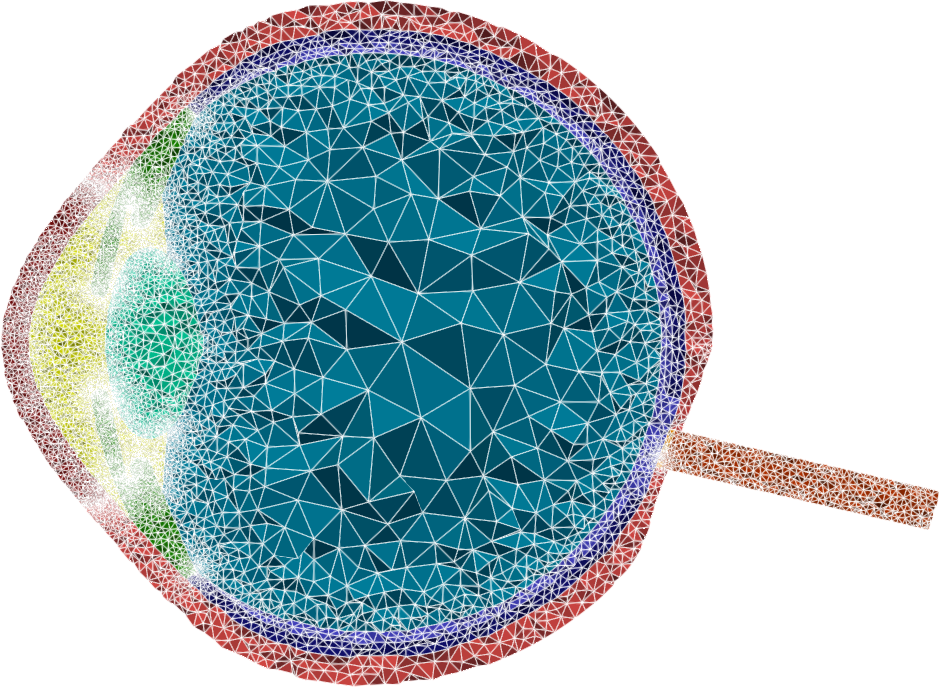
\includegraphics[width=0.6\textwidth]{feelpp/feelpp-benchmark-eyemesh.png}
  \caption{Mesh discretization, with the various regions of the eye.}
  \label{fig:spec:app-feelpp:eye2brain:mesh}
\end{figure}


%%%%%%%%%%%%%%%%%%%%%%%%%%%%%%%%%%%%%%%%%%%%%%%%%%%%%%%%%%%%%%%%%%%%%%%%%%%%%%%%%%%%%%%%%%%%%%%%%%%%%%%%%%%%%%%%%%%%%%%%


\subsection{Input/Output Dataset Description}


\subsubsection{Input Data:}
  \begin{itemize}
    \item Meshes: We have generated meshes of various level of refinement, denoted from \texttt{M2} to \texttt{M5}.
      The characteristics of the meshes, as well as the number of degree of freedom for various order of discretization is presented in \Cref{tab:spec:app-feelpp:eye2brain:mesh_stats}.
      All the meshes are pre-partitionned, with the application \texttt{feelpp\_mesh\_partitionner}\footnote{\url{https://docs.feelpp.org/user/latest/using/tools/mesh_partitioner.html}}
    \item Setup: use the function provided by the library \Feelpp, such as mesh manipulation and data exporter.
      The full source code is available in \texttt{src} directory of the GitHub repository \texttt{apps-feelpp}.
    \item Sif image: \texttt{feelpp:v0.111.0-preview.10-noble-sif}  (stored in the GitHub registry of \Feelpp)
  \end{itemize}

\SetTblrInner{rowsep=0pt}
\begin{table}[!ht]
    \centering
    \resizebox{\textwidth}{!}{
    \begin{tblr}{
        colspec={c*{9}{Q[c, cmd=\pgfmathprintnumber]}},
        vlines={numpexgray},
        hlines={numpexgray},
        row{1,2}={bg=numpexgray, fg=white, font=\bfseries, halign=c, cmd=\normalfont},
        rowhead=2,
    }
    \SetCell[c=4]{c}{Mesh properties} & & & & \SetCell[c=6]{c}{Number of degrees of freedom} & &\\
        Tag & \# points & \# edge & \# faces & $\mathP_1$ & $\mathP_2$ & $\mathP_3$ & $\mathP_4$ & $\mathP_5$ & $\mathP_6$ \\
        \texttt{M2} & 120581  & 762245   & 1273293  & 120581  & 882826   & 2918364   & 6858823   & 13335831  & 22981016 \\
        \texttt{M3} & 207845  & 1373087  & 2318292  & 207845  & 1580932  & 5272311   & 12435031  & 24222141  & 41786690 \\
        \texttt{M4} & 995906  & 6874446  & 11717323 & 995906  & 7870352  & 26462121  & 62609995  & 122152756 & 210929186 \\
        \texttt{M5} & 7360346 & 51295490 & 87714470 & 7360346 & 58655836 & 197665796 & 468169551 & 913946426 & 1578775746 \\
    \end{tblr}
    }

  \caption{Statistics on meshes of the eye and number of degrees of freedom with respect to finite element approximation.}
  \label{tab:spec:app-feelpp:eye2brain:mesh_stats}
\end{table}

\subsubsection{Output Data:}

The monitored quantities are the average times for each of the steps run in the loop described above:
\begin{inparaenum}[\it(i)]
\item \texttt{time\_loadMesh}, the time taken by the application to load the mesh from the disk;
\item \texttt{time\_createFunctionSpace}, the time taken to create the functional space $X_h$ or order $d$;
\item \texttt{time\_saveMesh}, the time taken to write the mesh data on the disk, in a new file;
\item \texttt{time\_export}, the time to export the vector $u\in X_h$ to disk, using the \texttt{exporter} functionality of \Feelpp.
\end{inparaenum}
The times are stored in a JSON file during execution.


%%%%%%%%%%%%%%%%%%%%%%%%%%%%%%%%%%%%%%%%%%%%%%%%%%%%%%%%%%%%%%%%%%%%%%%%%%%%%%%%%%%%%%%%%%%%%%%%%%%%%%%%%%%%%%%%%%%%%%%%

\subsection{Results summary}



We present in \Cref{fig:specs:app-feelpp-io:np} the results of execution of this benchmark over the family of mesh, for a various number of parallel tasks.
The mini-app is run on the cluster Gaya.
The results presented are obtained with the degree of discretization $\mathP_1$.
Similar behaviors are observed for other degree of discretization.

Note that some points are missing, either because the memory available on the nodes was too high for a node of Gaya, or because the iterative process described above took more than the time allocated to the job (1 hour).

We see that the steps of reading data and of creation of the functional spaces scale well according to the number of parallel process, as pointed out in \Cref{fig:specs:app-feelpp-io:np:loadmesh,fig:specs:app-feelpp-io:np:functionspace,fig:specs:app-feelpp-io:np:functionspaceV}, with a limit reached at $\texttt{np}=96$ for the small meshes.

On the contrary, the steps where we write data on the disk do not scale when the number of parallel process increases.
Precisely, this time gets higher, as pointed out in \Cref{fig:specs:app-feelpp-io:np:savemesh,fig:specs:app-feelpp-io:np:exportfield,fig:specs:app-feelpp-io:np:exportfieldv} or stagnated as shown in \Cref{fig:specs:app-feelpp-io:np:export}.
This loss of performance can be explained because of the communication of the parallel process that need to coordinate to write data on a single spot on disk.
As the mesh is already pre-partitionned, we do not have the same issue during the reading step.

\import{chapters/applications/specs/data/app-feelpp-io}{figure-np.tex}


\vspace{\baselineskip}

Now, we present in \Cref{fig:specs:app-feelpp-io:disc} the evolution of the time taken by each step, depending on the degree of discretization considered.
Specifically, we see in \Cref{fig:specs:app-feelpp-io:disc:loadmesh,fig:specs:app-feelpp-io:disc:savemesh} that the mesh manipulation is indeed independent of the degree of discretization.

On the contrary, the other steps are impacted by this degree, as it results in a higher number of degree of freedom, as shown in the mesh statistics in \Cref{tab:spec:app-feelpp:eye2brain:mesh_stats}.
Precisely, we see in \Cref{fig:specs:app-feelpp-io:disc:functionspace,fig:specs:app-feelpp-io:disc:functionspaceV} that the time increases linearly when the order increases, and that this raise of computational time is more important when the program write data on the disk, as shown in \Cref{fig:specs:app-feelpp-io:disc:exportfield,fig:specs:app-feelpp-io:disc:exportfieldv,fig:specs:app-feelpp-io:disc:export}.

\import{chapters/applications/specs/data/app-feelpp-io}{figure-order.tex}

